\documentclass[twoside]{book}

% Packages required by doxygen
\usepackage{fixltx2e}
\usepackage{calc}
\usepackage{doxygen}
\usepackage[export]{adjustbox} % also loads graphicx
\usepackage{graphicx}
\usepackage[utf8]{inputenc}
\usepackage{makeidx}
\usepackage{multicol}
\usepackage{multirow}
\PassOptionsToPackage{warn}{textcomp}
\usepackage{textcomp}
\usepackage[nointegrals]{wasysym}
\usepackage[table]{xcolor}

% Font selection
\usepackage[T1]{fontenc}
\usepackage[scaled=.90]{helvet}
\usepackage{courier}
\usepackage{amssymb}
\usepackage{sectsty}
\renewcommand{\familydefault}{\sfdefault}
\allsectionsfont{%
  \fontseries{bc}\selectfont%
  \color{darkgray}%
}
\renewcommand{\DoxyLabelFont}{%
  \fontseries{bc}\selectfont%
  \color{darkgray}%
}
\newcommand{\+}{\discretionary{\mbox{\scriptsize$\hookleftarrow$}}{}{}}

% Page & text layout
\usepackage{geometry}
\geometry{%
  a4paper,%
  top=2.5cm,%
  bottom=2.5cm,%
  left=2.5cm,%
  right=2.5cm%
}
\tolerance=750
\hfuzz=15pt
\hbadness=750
\setlength{\emergencystretch}{15pt}
\setlength{\parindent}{0cm}
\setlength{\parskip}{3ex plus 2ex minus 2ex}
\makeatletter
\renewcommand{\paragraph}{%
  \@startsection{paragraph}{4}{0ex}{-1.0ex}{1.0ex}{%
    \normalfont\normalsize\bfseries\SS@parafont%
  }%
}
\renewcommand{\subparagraph}{%
  \@startsection{subparagraph}{5}{0ex}{-1.0ex}{1.0ex}{%
    \normalfont\normalsize\bfseries\SS@subparafont%
  }%
}
\makeatother

% Headers & footers
\usepackage{fancyhdr}
\pagestyle{fancyplain}
\fancyhead[LE]{\fancyplain{}{\bfseries\thepage}}
\fancyhead[CE]{\fancyplain{}{}}
\fancyhead[RE]{\fancyplain{}{\bfseries\leftmark}}
\fancyhead[LO]{\fancyplain{}{\bfseries\rightmark}}
\fancyhead[CO]{\fancyplain{}{}}
\fancyhead[RO]{\fancyplain{}{\bfseries\thepage}}
\fancyfoot[LE]{\fancyplain{}{}}
\fancyfoot[CE]{\fancyplain{}{}}
\fancyfoot[RE]{\fancyplain{}{\bfseries\scriptsize Generated by Doxygen }}
\fancyfoot[LO]{\fancyplain{}{\bfseries\scriptsize Generated by Doxygen }}
\fancyfoot[CO]{\fancyplain{}{}}
\fancyfoot[RO]{\fancyplain{}{}}
\renewcommand{\footrulewidth}{0.4pt}
\renewcommand{\chaptermark}[1]{%
  \markboth{#1}{}%
}
\renewcommand{\sectionmark}[1]{%
  \markright{\thesection\ #1}%
}

% Indices & bibliography
\usepackage{natbib}
\usepackage[titles]{tocloft}
\setcounter{tocdepth}{3}
\setcounter{secnumdepth}{5}
\makeindex

% Hyperlinks (required, but should be loaded last)
\usepackage{ifpdf}
\ifpdf
  \usepackage[pdftex,pagebackref=true]{hyperref}
\else
  \usepackage[ps2pdf,pagebackref=true]{hyperref}
\fi
\hypersetup{%
  colorlinks=true,%
  linkcolor=blue,%
  citecolor=blue,%
  unicode%
}

% Custom commands
\newcommand{\clearemptydoublepage}{%
  \newpage{\pagestyle{empty}\cleardoublepage}%
}

\usepackage{caption}
\captionsetup{labelsep=space,justification=centering,font={bf},singlelinecheck=off,skip=4pt,position=top}

%===== C O N T E N T S =====

\begin{document}

% Titlepage & ToC
\hypersetup{pageanchor=false,
             bookmarksnumbered=true,
             pdfencoding=unicode
            }
\pagenumbering{roman}
\begin{titlepage}
\vspace*{7cm}
\begin{center}%
{\Large My Project }\\
\vspace*{1cm}
{\large Generated by Doxygen 1.8.11}\\
\end{center}
\end{titlepage}
\clearemptydoublepage
\tableofcontents
\clearemptydoublepage
\pagenumbering{arabic}
\hypersetup{pageanchor=true}

%--- Begin generated contents ---
\chapter{Class Index}
\section{Class List}
Here are the classes, structs, unions and interfaces with brief descriptions\+:\begin{DoxyCompactList}
\item\contentsline{section}{\hyperlink{structnode}{node} }{\pageref{structnode}}{}
\item\contentsline{section}{\hyperlink{structnode1}{node1} }{\pageref{structnode1}}{}
\item\contentsline{section}{\hyperlink{structnode__info}{node\+\_\+info} }{\pageref{structnode__info}}{}
\end{DoxyCompactList}

\chapter{File Index}
\section{File List}
Here is a list of all files with brief descriptions\+:\begin{DoxyCompactList}
\item\contentsline{section}{\hyperlink{Lab1_8c}{Lab1.\+c} }{\pageref{Lab1_8c}}{}
\end{DoxyCompactList}

\chapter{Class Documentation}
\hypertarget{structnode}{}\section{node Struct Reference}
\label{structnode}\index{node@{node}}


Collaboration diagram for node\+:
\nopagebreak
\begin{figure}[H]
\begin{center}
\leavevmode
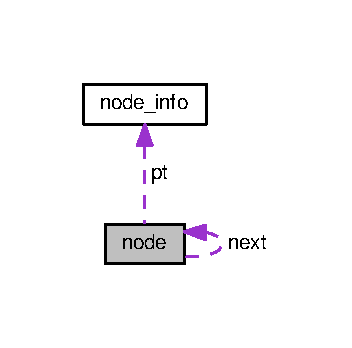
\includegraphics[width=158pt]{structnode__coll__graph}
\end{center}
\end{figure}
\subsection*{Public Attributes}
\begin{DoxyCompactItemize}
\item 
int \hyperlink{structnode_a2d890bb9f6af0ffd73fe79b21124c2a2}{data}
\item 
\hyperlink{structnode}{node} $\ast$ \hyperlink{structnode_aad210fa7c160a49f6b9a3ffee592a2bc}{next}
\end{DoxyCompactItemize}


\subsection{Member Data Documentation}
\index{node@{node}!data@{data}}
\index{data@{data}!node@{node}}
\subsubsection[{\texorpdfstring{data}{data}}]{\setlength{\rightskip}{0pt plus 5cm}int node\+::data}\hypertarget{structnode_a2d890bb9f6af0ffd73fe79b21124c2a2}{}\label{structnode_a2d890bb9f6af0ffd73fe79b21124c2a2}
\index{node@{node}!next@{next}}
\index{next@{next}!node@{node}}
\subsubsection[{\texorpdfstring{next}{next}}]{\setlength{\rightskip}{0pt plus 5cm}{\bf node}$\ast$ node\+::next}\hypertarget{structnode_aad210fa7c160a49f6b9a3ffee592a2bc}{}\label{structnode_aad210fa7c160a49f6b9a3ffee592a2bc}


The documentation for this struct was generated from the following file\+:\begin{DoxyCompactItemize}
\item 
\hyperlink{SelfOrganizing_8cpp}{Self\+Organizing.\+cpp}\end{DoxyCompactItemize}

\hypertarget{structnode1}{}\section{node1 Struct Reference}
\label{structnode1}\index{node1@{node1}}


Collaboration diagram for node1\+:
\nopagebreak
\begin{figure}[H]
\begin{center}
\leavevmode
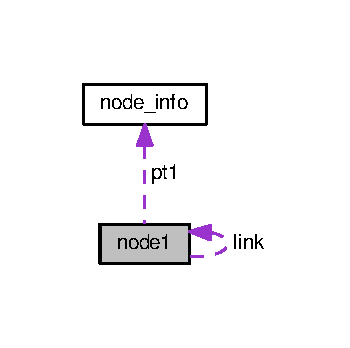
\includegraphics[width=169pt]{structnode1__coll__graph}
\end{center}
\end{figure}
\subsection*{Public Attributes}
\begin{DoxyCompactItemize}
\item 
int \hyperlink{structnode1_a3b6a50ecb2a2883e7a0a364ce108d2ad}{data1}
\item 
\hyperlink{structnode1}{node1} $\ast$ \hyperlink{structnode1_a91021c80c43acf0a49ffec9b73bf46ad}{next1}
\end{DoxyCompactItemize}


\subsection{Member Data Documentation}
\index{node1@{node1}!data1@{data1}}
\index{data1@{data1}!node1@{node1}}
\subsubsection[{\texorpdfstring{data1}{data1}}]{\setlength{\rightskip}{0pt plus 5cm}int node1\+::data1}\hypertarget{structnode1_a3b6a50ecb2a2883e7a0a364ce108d2ad}{}\label{structnode1_a3b6a50ecb2a2883e7a0a364ce108d2ad}
\index{node1@{node1}!next1@{next1}}
\index{next1@{next1}!node1@{node1}}
\subsubsection[{\texorpdfstring{next1}{next1}}]{\setlength{\rightskip}{0pt plus 5cm}{\bf node1}$\ast$ node1\+::next1}\hypertarget{structnode1_a91021c80c43acf0a49ffec9b73bf46ad}{}\label{structnode1_a91021c80c43acf0a49ffec9b73bf46ad}


The documentation for this struct was generated from the following file\+:\begin{DoxyCompactItemize}
\item 
\hyperlink{Hanoi_8cpp}{Hanoi.\+cpp}\end{DoxyCompactItemize}

\hypertarget{structnode__info}{}\section{node\+\_\+info Struct Reference}
\label{structnode__info}\index{node\+\_\+info@{node\+\_\+info}}
\subsection*{Public Attributes}
\begin{DoxyCompactItemize}
\item 
int \hyperlink{structnode__info_a69968058a534ead0624aeaf1428ed902}{no}
\item 
int \hyperlink{structnode__info_a85fd243a529e8b5387e2f744ec6f0ab1}{lv\+\_\+time}
\item 
int \hyperlink{structnode__info_a303996389f9a5755e0ddd41faa3eb987}{st\+\_\+time}
\end{DoxyCompactItemize}


\subsection{Member Data Documentation}
\index{node\+\_\+info@{node\+\_\+info}!lv\+\_\+time@{lv\+\_\+time}}
\index{lv\+\_\+time@{lv\+\_\+time}!node\+\_\+info@{node\+\_\+info}}
\subsubsection[{\texorpdfstring{lv\+\_\+time}{lv_time}}]{\setlength{\rightskip}{0pt plus 5cm}int node\+\_\+info\+::lv\+\_\+time}\hypertarget{structnode__info_a85fd243a529e8b5387e2f744ec6f0ab1}{}\label{structnode__info_a85fd243a529e8b5387e2f744ec6f0ab1}
\index{node\+\_\+info@{node\+\_\+info}!no@{no}}
\index{no@{no}!node\+\_\+info@{node\+\_\+info}}
\subsubsection[{\texorpdfstring{no}{no}}]{\setlength{\rightskip}{0pt plus 5cm}int node\+\_\+info\+::no}\hypertarget{structnode__info_a69968058a534ead0624aeaf1428ed902}{}\label{structnode__info_a69968058a534ead0624aeaf1428ed902}
\index{node\+\_\+info@{node\+\_\+info}!st\+\_\+time@{st\+\_\+time}}
\index{st\+\_\+time@{st\+\_\+time}!node\+\_\+info@{node\+\_\+info}}
\subsubsection[{\texorpdfstring{st\+\_\+time}{st_time}}]{\setlength{\rightskip}{0pt plus 5cm}int node\+\_\+info\+::st\+\_\+time}\hypertarget{structnode__info_a303996389f9a5755e0ddd41faa3eb987}{}\label{structnode__info_a303996389f9a5755e0ddd41faa3eb987}


The documentation for this struct was generated from the following file\+:\begin{DoxyCompactItemize}
\item 
\hyperlink{ConenctedGraph_8cpp}{Conencted\+Graph.\+cpp}\end{DoxyCompactItemize}

\chapter{File Documentation}
\hypertarget{ConenctedGraph_8cpp}{}\section{Conencted\+Graph.\+cpp File Reference}
\label{ConenctedGraph_8cpp}\index{Conencted\+Graph.\+cpp@{Conencted\+Graph.\+cpp}}
{\ttfamily \#include $<$iostream$>$}\\*
{\ttfamily \#include $<$conio.\+h$>$}\\*
Include dependency graph for Conencted\+Graph.\+cpp\+:
\nopagebreak
\begin{figure}[H]
\begin{center}
\leavevmode
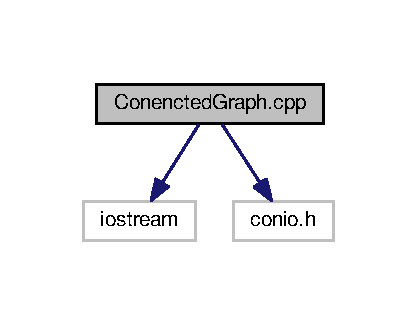
\includegraphics[width=200pt]{ConenctedGraph_8cpp__incl}
\end{center}
\end{figure}
\subsection*{Classes}
\begin{DoxyCompactItemize}
\item 
struct \hyperlink{structnode__info}{node\+\_\+info}
\item 
struct \hyperlink{structnode}{node}
\item 
struct \hyperlink{structnode1}{node1}
\end{DoxyCompactItemize}
\subsection*{Functions}
\begin{DoxyCompactItemize}
\item 
void \hyperlink{ConenctedGraph_8cpp_aae451c1ebd106d944a840164e8db9514}{push} (\hyperlink{structnode__info}{node\+\_\+info} $\ast$ptr)
\item 
\hyperlink{structnode__info}{node\+\_\+info} $\ast$ \hyperlink{ConenctedGraph_8cpp_ae9aa7e778dbc81f5869b4d2909f08cdc}{pop} ()
\item 
void \hyperlink{ConenctedGraph_8cpp_a60d767824e49bbfd6b355613c5cf688b}{store} (\hyperlink{structnode__info}{node\+\_\+info} $\ast$ptr1)
\item 
void \hyperlink{ConenctedGraph_8cpp_af687fb1dfedb0616384c2365c60a6df6}{remove} (int x)
\item 
void \hyperlink{ConenctedGraph_8cpp_a94241e7f0ac74dc536b674ae552c5514}{topo} (int $\ast$v, int am\mbox{[}$\,$\mbox{]}\mbox{[}8\mbox{]}, int i)
\item 
void \hyperlink{ConenctedGraph_8cpp_a89339819b5c1f956c3cb7ffcc8c87527}{topo1} (int $\ast$v, int am\mbox{[}$\,$\mbox{]}\mbox{[}8\mbox{]}, int i)
\item 
int \hyperlink{ConenctedGraph_8cpp_ae66f6b31b5ad750f1fe042a706a4e3d4}{main} ()
\end{DoxyCompactItemize}
\subsection*{Variables}
\begin{DoxyCompactItemize}
\item 
struct \hyperlink{structnode__info}{node\+\_\+info} $\ast$ \hyperlink{ConenctedGraph_8cpp_a165a4097380d255de91c05ce20db3d95}{q} = N\+U\+LL
\item 
struct \hyperlink{structnode}{node} $\ast$ \hyperlink{ConenctedGraph_8cpp_a6d07aa6ea9a4f27c003e8d4a546cab3c}{top} = N\+U\+LL
\item 
struct \hyperlink{structnode}{node} $\ast$ \hyperlink{ConenctedGraph_8cpp_a9a74b89eccf4182238b50fade064e20c}{p} = N\+U\+LL
\item 
struct \hyperlink{structnode}{node} $\ast$ \hyperlink{ConenctedGraph_8cpp_af9a416d5a2fbb97692e019ed4922c1fb}{np} = N\+U\+LL
\item 
struct \hyperlink{structnode1}{node1} $\ast$ \hyperlink{ConenctedGraph_8cpp_ad14537846bc32b6576ef92ef28b0a7db}{head} = N\+U\+LL
\item 
struct \hyperlink{structnode1}{node1} $\ast$ \hyperlink{ConenctedGraph_8cpp_a7b67eeec44d92b5971d5198ea27046ae}{m} = N\+U\+LL
\item 
struct \hyperlink{structnode1}{node1} $\ast$ \hyperlink{ConenctedGraph_8cpp_a7f99fd69932220e7650dc832bd6d8015}{n} = N\+U\+LL
\item 
struct \hyperlink{structnode1}{node1} $\ast$ \hyperlink{ConenctedGraph_8cpp_af2631d988504474b2e0882737b7bb156}{np1} = N\+U\+LL
\item 
int \hyperlink{ConenctedGraph_8cpp_a4e1e0e72dd773439e333c84dd762a9c3}{c} = 0
\end{DoxyCompactItemize}


\subsection{Function Documentation}
\index{Conencted\+Graph.\+cpp@{Conencted\+Graph.\+cpp}!main@{main}}
\index{main@{main}!Conencted\+Graph.\+cpp@{Conencted\+Graph.\+cpp}}
\subsubsection[{\texorpdfstring{main()}{main()}}]{\setlength{\rightskip}{0pt plus 5cm}int main (
\begin{DoxyParamCaption}
{}
\end{DoxyParamCaption}
)}\hypertarget{ConenctedGraph_8cpp_ae66f6b31b5ad750f1fe042a706a4e3d4}{}\label{ConenctedGraph_8cpp_ae66f6b31b5ad750f1fe042a706a4e3d4}

\begin{DoxyCode}
139 \{
140     \textcolor{keywordtype}{int} v[8], am[8][8], amt[8][8];
141     \textcolor{keywordflow}{for} (\textcolor{keywordtype}{int} i = 0; i < 8; i++)
142         v[i] = 0;
143     \textcolor{keywordflow}{for} (\textcolor{keywordtype}{int} i = 0; i < 8; i++)
144     \{
145         cout<<\textcolor{stringliteral}{"enter the values for adjacency matrix row:"}<<i + 1<<endl;
146         \textcolor{keywordflow}{for} (\textcolor{keywordtype}{int} j = 0; j < 8; j++)
147         \{
148             cin>>am[i][j];
149         \}
150     \}
151     \hyperlink{ConenctedGraph_8cpp_a94241e7f0ac74dc536b674ae552c5514}{topo}(v, am, 0);
152     \textcolor{keywordflow}{for} (\textcolor{keywordtype}{int} i = 0; i < 8; i++)
153     \{
154         v[i] = 0;
155         \textcolor{keywordflow}{for} (\textcolor{keywordtype}{int} j = 0; j < 8; j++)
156             amt[j][i] = am[i][j];
157     \}
158     \textcolor{keywordflow}{while} (\hyperlink{ConenctedGraph_8cpp_ad14537846bc32b6576ef92ef28b0a7db}{head} != NULL)
159     \{
160         cout<<\textcolor{stringliteral}{"Strongly Connected Components:\(\backslash\)n"};                 
161             \hyperlink{ConenctedGraph_8cpp_a89339819b5c1f956c3cb7ffcc8c87527}{topo1}(v, amt, (\hyperlink{ConenctedGraph_8cpp_ad14537846bc32b6576ef92ef28b0a7db}{head}->\hyperlink{structnode1_a6c3bc0362d5ce74f576c735c17747b28}{pt1})->no);
162     \}
163     getch();
164 \}\end{DoxyCode}


Here is the call graph for this function\+:
\nopagebreak
\begin{figure}[H]
\begin{center}
\leavevmode
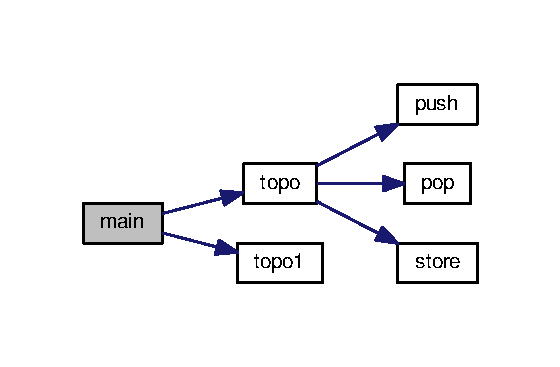
\includegraphics[width=269pt]{ConenctedGraph_8cpp_ae66f6b31b5ad750f1fe042a706a4e3d4_cgraph}
\end{center}
\end{figure}


\index{Conencted\+Graph.\+cpp@{Conencted\+Graph.\+cpp}!pop@{pop}}
\index{pop@{pop}!Conencted\+Graph.\+cpp@{Conencted\+Graph.\+cpp}}
\subsubsection[{\texorpdfstring{pop()}{pop()}}]{\setlength{\rightskip}{0pt plus 5cm}{\bf node\+\_\+info}$\ast$ pop (
\begin{DoxyParamCaption}
{}
\end{DoxyParamCaption}
)}\hypertarget{ConenctedGraph_8cpp_ae9aa7e778dbc81f5869b4d2909f08cdc}{}\label{ConenctedGraph_8cpp_ae9aa7e778dbc81f5869b4d2909f08cdc}

\begin{DoxyCode}
39 \{
40     \textcolor{keywordflow}{if} (\hyperlink{ConenctedGraph_8cpp_a6d07aa6ea9a4f27c003e8d4a546cab3c}{top} == NULL)
41     \{
42         cout<<\textcolor{stringliteral}{"underflow\(\backslash\)n"};
43     \}
44     \textcolor{keywordflow}{else}
45     \{
46         \hyperlink{ConenctedGraph_8cpp_a9a74b89eccf4182238b50fade064e20c}{p} = \hyperlink{ConenctedGraph_8cpp_a6d07aa6ea9a4f27c003e8d4a546cab3c}{top};
47         \hyperlink{ConenctedGraph_8cpp_a6d07aa6ea9a4f27c003e8d4a546cab3c}{top} = \hyperlink{ConenctedGraph_8cpp_a6d07aa6ea9a4f27c003e8d4a546cab3c}{top}->\hyperlink{structnode_aad210fa7c160a49f6b9a3ffee592a2bc}{next};
48         \textcolor{keywordflow}{return}(\hyperlink{ConenctedGraph_8cpp_a9a74b89eccf4182238b50fade064e20c}{p}->\hyperlink{structnode_ad5d98c32ab86154ae188cbdd5dca64a3}{pt});
49         \textcolor{keyword}{delete}(\hyperlink{ConenctedGraph_8cpp_a9a74b89eccf4182238b50fade064e20c}{p});
50     \}
51 \}
\end{DoxyCode}
\index{Conencted\+Graph.\+cpp@{Conencted\+Graph.\+cpp}!push@{push}}
\index{push@{push}!Conencted\+Graph.\+cpp@{Conencted\+Graph.\+cpp}}
\subsubsection[{\texorpdfstring{push(node\+\_\+info $\ast$ptr)}{push(node_info *ptr)}}]{\setlength{\rightskip}{0pt plus 5cm}void push (
\begin{DoxyParamCaption}
\item[{{\bf node\+\_\+info} $\ast$}]{ptr}
\end{DoxyParamCaption}
)}\hypertarget{ConenctedGraph_8cpp_aae451c1ebd106d944a840164e8db9514}{}\label{ConenctedGraph_8cpp_aae451c1ebd106d944a840164e8db9514}

\begin{DoxyCode}
24 \{
25     \hyperlink{ConenctedGraph_8cpp_af9a416d5a2fbb97692e019ed4922c1fb}{np} = \textcolor{keyword}{new} \hyperlink{structnode}{node};
26     \hyperlink{ConenctedGraph_8cpp_af9a416d5a2fbb97692e019ed4922c1fb}{np}->\hyperlink{structnode_ad5d98c32ab86154ae188cbdd5dca64a3}{pt} = ptr;
27     \hyperlink{ConenctedGraph_8cpp_af9a416d5a2fbb97692e019ed4922c1fb}{np}->\hyperlink{structnode_aad210fa7c160a49f6b9a3ffee592a2bc}{next} = NULL;
28     \textcolor{keywordflow}{if} (\hyperlink{ConenctedGraph_8cpp_a6d07aa6ea9a4f27c003e8d4a546cab3c}{top} == NULL)
29     \{
30         \hyperlink{ConenctedGraph_8cpp_a6d07aa6ea9a4f27c003e8d4a546cab3c}{top} = \hyperlink{ConenctedGraph_8cpp_af9a416d5a2fbb97692e019ed4922c1fb}{np};
31     \}
32     \textcolor{keywordflow}{else}
33     \{
34         \hyperlink{ConenctedGraph_8cpp_af9a416d5a2fbb97692e019ed4922c1fb}{np}->\hyperlink{structnode_aad210fa7c160a49f6b9a3ffee592a2bc}{next} = \hyperlink{ConenctedGraph_8cpp_a6d07aa6ea9a4f27c003e8d4a546cab3c}{top};
35         \hyperlink{ConenctedGraph_8cpp_a6d07aa6ea9a4f27c003e8d4a546cab3c}{top} = \hyperlink{ConenctedGraph_8cpp_af9a416d5a2fbb97692e019ed4922c1fb}{np};
36     \}
37 \}
\end{DoxyCode}
\index{Conencted\+Graph.\+cpp@{Conencted\+Graph.\+cpp}!remove@{remove}}
\index{remove@{remove}!Conencted\+Graph.\+cpp@{Conencted\+Graph.\+cpp}}
\subsubsection[{\texorpdfstring{remove(int x)}{remove(int x)}}]{\setlength{\rightskip}{0pt plus 5cm}void remove (
\begin{DoxyParamCaption}
\item[{int}]{x}
\end{DoxyParamCaption}
)}\hypertarget{ConenctedGraph_8cpp_af687fb1dfedb0616384c2365c60a6df6}{}\label{ConenctedGraph_8cpp_af687fb1dfedb0616384c2365c60a6df6}

\begin{DoxyCode}
72 \{
73     \hyperlink{ConenctedGraph_8cpp_a7b67eeec44d92b5971d5198ea27046ae}{m} = \hyperlink{ConenctedGraph_8cpp_ad14537846bc32b6576ef92ef28b0a7db}{head};
74     \textcolor{keywordflow}{if} ((\hyperlink{ConenctedGraph_8cpp_a7b67eeec44d92b5971d5198ea27046ae}{m}->\hyperlink{structnode1_a6c3bc0362d5ce74f576c735c17747b28}{pt1})->no == x)
75     \{
76         \hyperlink{ConenctedGraph_8cpp_ad14537846bc32b6576ef92ef28b0a7db}{head} = \hyperlink{ConenctedGraph_8cpp_ad14537846bc32b6576ef92ef28b0a7db}{head}->\hyperlink{structnode1_a7c5f011dde8e80cc5a24a5fad943138d}{link};
77         \textcolor{keyword}{delete}(\hyperlink{ConenctedGraph_8cpp_a7b67eeec44d92b5971d5198ea27046ae}{m});
78     \}
79     \textcolor{keywordflow}{else}
80     \{
81         \textcolor{keywordflow}{while} ((\hyperlink{ConenctedGraph_8cpp_a7b67eeec44d92b5971d5198ea27046ae}{m}->\hyperlink{structnode1_a6c3bc0362d5ce74f576c735c17747b28}{pt1})->no != x && \hyperlink{ConenctedGraph_8cpp_a7b67eeec44d92b5971d5198ea27046ae}{m}->\hyperlink{structnode1_a7c5f011dde8e80cc5a24a5fad943138d}{link} != NULL)
82         \{
83             \hyperlink{ConenctedGraph_8cpp_a7f99fd69932220e7650dc832bd6d8015}{n} = \hyperlink{ConenctedGraph_8cpp_a7b67eeec44d92b5971d5198ea27046ae}{m};
84             \hyperlink{ConenctedGraph_8cpp_a7b67eeec44d92b5971d5198ea27046ae}{m} = \hyperlink{ConenctedGraph_8cpp_a7b67eeec44d92b5971d5198ea27046ae}{m}->\hyperlink{structnode1_a7c5f011dde8e80cc5a24a5fad943138d}{link};
85         \}
86         \textcolor{keywordflow}{if} ((\hyperlink{ConenctedGraph_8cpp_a7b67eeec44d92b5971d5198ea27046ae}{m}->\hyperlink{structnode1_a6c3bc0362d5ce74f576c735c17747b28}{pt1})->no == x)
87         \{
88             \hyperlink{ConenctedGraph_8cpp_a7f99fd69932220e7650dc832bd6d8015}{n}->\hyperlink{structnode1_a7c5f011dde8e80cc5a24a5fad943138d}{link} = \hyperlink{ConenctedGraph_8cpp_a7b67eeec44d92b5971d5198ea27046ae}{m}->\hyperlink{structnode1_a7c5f011dde8e80cc5a24a5fad943138d}{link};
89             \textcolor{keyword}{delete}(\hyperlink{ConenctedGraph_8cpp_a7b67eeec44d92b5971d5198ea27046ae}{m});
90         \}
91         \textcolor{keywordflow}{else} \textcolor{keywordflow}{if} (\hyperlink{ConenctedGraph_8cpp_a7b67eeec44d92b5971d5198ea27046ae}{m}->\hyperlink{structnode1_a7c5f011dde8e80cc5a24a5fad943138d}{link} == NULL)
92         \{
93             cout<<\textcolor{stringliteral}{"error\(\backslash\)n"};
94         \}
95     \}
96 \}            
\end{DoxyCode}
\index{Conencted\+Graph.\+cpp@{Conencted\+Graph.\+cpp}!store@{store}}
\index{store@{store}!Conencted\+Graph.\+cpp@{Conencted\+Graph.\+cpp}}
\subsubsection[{\texorpdfstring{store(node\+\_\+info $\ast$ptr1)}{store(node_info *ptr1)}}]{\setlength{\rightskip}{0pt plus 5cm}void store (
\begin{DoxyParamCaption}
\item[{{\bf node\+\_\+info} $\ast$}]{ptr1}
\end{DoxyParamCaption}
)}\hypertarget{ConenctedGraph_8cpp_a60d767824e49bbfd6b355613c5cf688b}{}\label{ConenctedGraph_8cpp_a60d767824e49bbfd6b355613c5cf688b}

\begin{DoxyCode}
53 \{
54     \hyperlink{ConenctedGraph_8cpp_af2631d988504474b2e0882737b7bb156}{np1} = \textcolor{keyword}{new} \hyperlink{structnode1}{node1};
55     \hyperlink{ConenctedGraph_8cpp_af2631d988504474b2e0882737b7bb156}{np1}->\hyperlink{structnode1_a6c3bc0362d5ce74f576c735c17747b28}{pt1} = ptr1;
56     \hyperlink{ConenctedGraph_8cpp_af2631d988504474b2e0882737b7bb156}{np1}->\hyperlink{structnode1_a7c5f011dde8e80cc5a24a5fad943138d}{link} = NULL;
57     \textcolor{keywordflow}{if} (\hyperlink{ConenctedGraph_8cpp_a4e1e0e72dd773439e333c84dd762a9c3}{c} == 0)
58     \{
59         \hyperlink{ConenctedGraph_8cpp_ad14537846bc32b6576ef92ef28b0a7db}{head} = \hyperlink{ConenctedGraph_8cpp_af2631d988504474b2e0882737b7bb156}{np1};
60         \hyperlink{ConenctedGraph_8cpp_a7b67eeec44d92b5971d5198ea27046ae}{m} = \hyperlink{ConenctedGraph_8cpp_ad14537846bc32b6576ef92ef28b0a7db}{head};
61         \hyperlink{ConenctedGraph_8cpp_a7b67eeec44d92b5971d5198ea27046ae}{m}->\hyperlink{structnode1_a7c5f011dde8e80cc5a24a5fad943138d}{link} = NULL;
62         \hyperlink{ConenctedGraph_8cpp_a4e1e0e72dd773439e333c84dd762a9c3}{c}++;
63     \}
64     \textcolor{keywordflow}{else}
65     \{
66         \hyperlink{ConenctedGraph_8cpp_a7b67eeec44d92b5971d5198ea27046ae}{m} = \hyperlink{ConenctedGraph_8cpp_ad14537846bc32b6576ef92ef28b0a7db}{head};
67         \hyperlink{ConenctedGraph_8cpp_af2631d988504474b2e0882737b7bb156}{np1}->\hyperlink{structnode1_a7c5f011dde8e80cc5a24a5fad943138d}{link} = \hyperlink{ConenctedGraph_8cpp_a7b67eeec44d92b5971d5198ea27046ae}{m};
68         \hyperlink{ConenctedGraph_8cpp_ad14537846bc32b6576ef92ef28b0a7db}{head} = \hyperlink{ConenctedGraph_8cpp_af2631d988504474b2e0882737b7bb156}{np1};
69     \}
70 \}
\end{DoxyCode}
\index{Conencted\+Graph.\+cpp@{Conencted\+Graph.\+cpp}!topo@{topo}}
\index{topo@{topo}!Conencted\+Graph.\+cpp@{Conencted\+Graph.\+cpp}}
\subsubsection[{\texorpdfstring{topo(int $\ast$v, int am[][8], int i)}{topo(int *v, int am[][8], int i)}}]{\setlength{\rightskip}{0pt plus 5cm}void topo (
\begin{DoxyParamCaption}
\item[{int $\ast$}]{v, }
\item[{int}]{am\mbox{[}$\,$\mbox{]}\mbox{[}8\mbox{]}, }
\item[{int}]{i}
\end{DoxyParamCaption}
)}\hypertarget{ConenctedGraph_8cpp_a94241e7f0ac74dc536b674ae552c5514}{}\label{ConenctedGraph_8cpp_a94241e7f0ac74dc536b674ae552c5514}

\begin{DoxyCode}
98 \{
99     \hyperlink{ConenctedGraph_8cpp_a165a4097380d255de91c05ce20db3d95}{q} = \textcolor{keyword}{new} \hyperlink{structnode__info}{node\_info};
100     \hyperlink{ConenctedGraph_8cpp_a165a4097380d255de91c05ce20db3d95}{q}->\hyperlink{structnode__info_a69968058a534ead0624aeaf1428ed902}{no} = i;
101     \hyperlink{ConenctedGraph_8cpp_a165a4097380d255de91c05ce20db3d95}{q}->\hyperlink{structnode__info_a303996389f9a5755e0ddd41faa3eb987}{st\_time} = \hyperlink{ConenctedGraph_8cpp_a4e1e0e72dd773439e333c84dd762a9c3}{c};
102      \hyperlink{ConenctedGraph_8cpp_aae451c1ebd106d944a840164e8db9514}{push}(\hyperlink{ConenctedGraph_8cpp_a165a4097380d255de91c05ce20db3d95}{q});
103     v[i] = 1;
104     \textcolor{keywordflow}{for} (\textcolor{keywordtype}{int} j = 0; j < 8; j++)
105     \{
106         \textcolor{keywordflow}{if} (am[i][j] == 0  || (am[i][j] == 1 && v[j] == 1))
107             \textcolor{keywordflow}{continue};
108         \textcolor{keywordflow}{else} \textcolor{keywordflow}{if} (am[i][j] == 1 && v[j] == 0)
109         \{
110             \hyperlink{ConenctedGraph_8cpp_a4e1e0e72dd773439e333c84dd762a9c3}{c}++;
111             \hyperlink{ConenctedGraph_8cpp_a94241e7f0ac74dc536b674ae552c5514}{topo}(v,am,j);
112         \}
113     \}
114     \hyperlink{ConenctedGraph_8cpp_a4e1e0e72dd773439e333c84dd762a9c3}{c}++;
115     \hyperlink{ConenctedGraph_8cpp_a165a4097380d255de91c05ce20db3d95}{q} = \hyperlink{ConenctedGraph_8cpp_ae9aa7e778dbc81f5869b4d2909f08cdc}{pop}();
116     \hyperlink{ConenctedGraph_8cpp_a165a4097380d255de91c05ce20db3d95}{q}->\hyperlink{structnode__info_a85fd243a529e8b5387e2f744ec6f0ab1}{lv\_time} = \hyperlink{ConenctedGraph_8cpp_a4e1e0e72dd773439e333c84dd762a9c3}{c};
117     \hyperlink{ConenctedGraph_8cpp_a60d767824e49bbfd6b355613c5cf688b}{store}(\hyperlink{ConenctedGraph_8cpp_a165a4097380d255de91c05ce20db3d95}{q});
118     \textcolor{keywordflow}{return};
119 \}
\end{DoxyCode}


Here is the call graph for this function\+:
\nopagebreak
\begin{figure}[H]
\begin{center}
\leavevmode
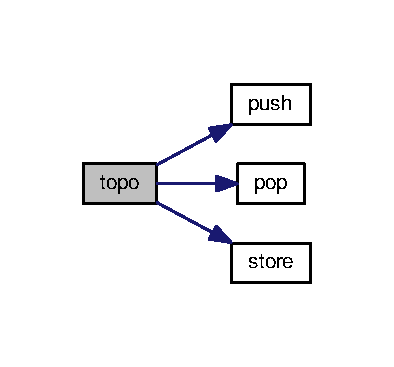
\includegraphics[width=189pt]{ConenctedGraph_8cpp_a94241e7f0ac74dc536b674ae552c5514_cgraph}
\end{center}
\end{figure}


\index{Conencted\+Graph.\+cpp@{Conencted\+Graph.\+cpp}!topo1@{topo1}}
\index{topo1@{topo1}!Conencted\+Graph.\+cpp@{Conencted\+Graph.\+cpp}}
\subsubsection[{\texorpdfstring{topo1(int $\ast$v, int am[][8], int i)}{topo1(int *v, int am[][8], int i)}}]{\setlength{\rightskip}{0pt plus 5cm}void topo1 (
\begin{DoxyParamCaption}
\item[{int $\ast$}]{v, }
\item[{int}]{am\mbox{[}$\,$\mbox{]}\mbox{[}8\mbox{]}, }
\item[{int}]{i}
\end{DoxyParamCaption}
)}\hypertarget{ConenctedGraph_8cpp_a89339819b5c1f956c3cb7ffcc8c87527}{}\label{ConenctedGraph_8cpp_a89339819b5c1f956c3cb7ffcc8c87527}

\begin{DoxyCode}
121 \{
122     v[i] = 1;
123     \textcolor{keyword}{remove}(i);
124     cout<<i<<endl;
125     \textcolor{keywordflow}{for} (\textcolor{keywordtype}{int} j = 0; j < 8; j++)
126     \{
127         \textcolor{keywordflow}{if} (am[i][j] == 0  || (am[i][j] == 1 && v[j] == 1))
128         \{
129             \textcolor{keywordflow}{continue};
130         \}
131         \textcolor{keywordflow}{else} \textcolor{keywordflow}{if} (am[i][j] == 1 && v[j] == 0)
132         \{
133             \hyperlink{ConenctedGraph_8cpp_a89339819b5c1f956c3cb7ffcc8c87527}{topo1}(v,am,j);
134         \}
135     \}
136     \textcolor{keywordflow}{return};
137 \}
\end{DoxyCode}


\subsection{Variable Documentation}
\index{Conencted\+Graph.\+cpp@{Conencted\+Graph.\+cpp}!c@{c}}
\index{c@{c}!Conencted\+Graph.\+cpp@{Conencted\+Graph.\+cpp}}
\subsubsection[{\texorpdfstring{c}{c}}]{\setlength{\rightskip}{0pt plus 5cm}int c = 0}\hypertarget{ConenctedGraph_8cpp_a4e1e0e72dd773439e333c84dd762a9c3}{}\label{ConenctedGraph_8cpp_a4e1e0e72dd773439e333c84dd762a9c3}
\index{Conencted\+Graph.\+cpp@{Conencted\+Graph.\+cpp}!head@{head}}
\index{head@{head}!Conencted\+Graph.\+cpp@{Conencted\+Graph.\+cpp}}
\subsubsection[{\texorpdfstring{head}{head}}]{\setlength{\rightskip}{0pt plus 5cm}struct {\bf node1}$\ast$ head = N\+U\+LL}\hypertarget{ConenctedGraph_8cpp_ad14537846bc32b6576ef92ef28b0a7db}{}\label{ConenctedGraph_8cpp_ad14537846bc32b6576ef92ef28b0a7db}
\index{Conencted\+Graph.\+cpp@{Conencted\+Graph.\+cpp}!m@{m}}
\index{m@{m}!Conencted\+Graph.\+cpp@{Conencted\+Graph.\+cpp}}
\subsubsection[{\texorpdfstring{m}{m}}]{\setlength{\rightskip}{0pt plus 5cm}struct {\bf node1} $\ast$ m = N\+U\+LL}\hypertarget{ConenctedGraph_8cpp_a7b67eeec44d92b5971d5198ea27046ae}{}\label{ConenctedGraph_8cpp_a7b67eeec44d92b5971d5198ea27046ae}
\index{Conencted\+Graph.\+cpp@{Conencted\+Graph.\+cpp}!n@{n}}
\index{n@{n}!Conencted\+Graph.\+cpp@{Conencted\+Graph.\+cpp}}
\subsubsection[{\texorpdfstring{n}{n}}]{\setlength{\rightskip}{0pt plus 5cm}struct {\bf node1} $\ast$ n = N\+U\+LL}\hypertarget{ConenctedGraph_8cpp_a7f99fd69932220e7650dc832bd6d8015}{}\label{ConenctedGraph_8cpp_a7f99fd69932220e7650dc832bd6d8015}
\index{Conencted\+Graph.\+cpp@{Conencted\+Graph.\+cpp}!np@{np}}
\index{np@{np}!Conencted\+Graph.\+cpp@{Conencted\+Graph.\+cpp}}
\subsubsection[{\texorpdfstring{np}{np}}]{\setlength{\rightskip}{0pt plus 5cm}struct {\bf node} $\ast$ np = N\+U\+LL}\hypertarget{ConenctedGraph_8cpp_af9a416d5a2fbb97692e019ed4922c1fb}{}\label{ConenctedGraph_8cpp_af9a416d5a2fbb97692e019ed4922c1fb}
\index{Conencted\+Graph.\+cpp@{Conencted\+Graph.\+cpp}!np1@{np1}}
\index{np1@{np1}!Conencted\+Graph.\+cpp@{Conencted\+Graph.\+cpp}}
\subsubsection[{\texorpdfstring{np1}{np1}}]{\setlength{\rightskip}{0pt plus 5cm}struct {\bf node1} $\ast$ np1 = N\+U\+LL}\hypertarget{ConenctedGraph_8cpp_af2631d988504474b2e0882737b7bb156}{}\label{ConenctedGraph_8cpp_af2631d988504474b2e0882737b7bb156}
\index{Conencted\+Graph.\+cpp@{Conencted\+Graph.\+cpp}!p@{p}}
\index{p@{p}!Conencted\+Graph.\+cpp@{Conencted\+Graph.\+cpp}}
\subsubsection[{\texorpdfstring{p}{p}}]{\setlength{\rightskip}{0pt plus 5cm}struct {\bf node} $\ast$ p = N\+U\+LL}\hypertarget{ConenctedGraph_8cpp_a9a74b89eccf4182238b50fade064e20c}{}\label{ConenctedGraph_8cpp_a9a74b89eccf4182238b50fade064e20c}
\index{Conencted\+Graph.\+cpp@{Conencted\+Graph.\+cpp}!q@{q}}
\index{q@{q}!Conencted\+Graph.\+cpp@{Conencted\+Graph.\+cpp}}
\subsubsection[{\texorpdfstring{q}{q}}]{\setlength{\rightskip}{0pt plus 5cm}struct {\bf node\+\_\+info}$\ast$ q = N\+U\+LL}\hypertarget{ConenctedGraph_8cpp_a165a4097380d255de91c05ce20db3d95}{}\label{ConenctedGraph_8cpp_a165a4097380d255de91c05ce20db3d95}
\index{Conencted\+Graph.\+cpp@{Conencted\+Graph.\+cpp}!top@{top}}
\index{top@{top}!Conencted\+Graph.\+cpp@{Conencted\+Graph.\+cpp}}
\subsubsection[{\texorpdfstring{top}{top}}]{\setlength{\rightskip}{0pt plus 5cm}struct {\bf node}$\ast$ top = N\+U\+LL}\hypertarget{ConenctedGraph_8cpp_a6d07aa6ea9a4f27c003e8d4a546cab3c}{}\label{ConenctedGraph_8cpp_a6d07aa6ea9a4f27c003e8d4a546cab3c}

%--- End generated contents ---

% Index
\backmatter
\newpage
\phantomsection
\clearemptydoublepage
\addcontentsline{toc}{chapter}{Index}
\printindex

\end{document}
